\section{Baselines and Methods}
\label{sec:exp}

%% 1. 简要再次介绍数据集

%\subsection{Dataset Splits}
The data for all experiments comes from UAV-BD. In order to ensure that the distributions of training and testing data approximately match, we randomly select $ 64\% $ of the UAV-BD as the training data, $ 16\% $ as validation data, and $ 20\% $ as the testing data. The whole UAV-BD contains $ 16258 $ images with $ 22211 $ instances for training, $ 5081 $ images with $ 6944 $ instances for testing and $ 4055 $ images with $ 5624 $ instances for validation. All the original images and segmented images with ground truth for UAV-BD will be publicly available.

%% 2. 实验使用了 4 中基于深度学习的方法

Here, we compare four kinds of approaches which differ in the use of detection framework and data annotating method. For horizontal object detection, we select Faster R-CNN\footnote{\url{https://github.com/rbgirshick/py-faster-rcnn.git}}\cite{FasterRCNN},  SSD\footnote{\url{https://github.com/weiliu89/caffe.git}}\cite{SSD} and YOLOv2\footnote{\url{https://pjreddie.com/darknet/yolo/}}\cite{YOLOv2} as our baseline testing algorithms for their excellent performance on general object detection. For oriented object detection, we modify the original Rotation Region Proposal Networks(RRPN\footnote{\url{https://github.com/mjq11302010044/RRPN.git}}) algorithm\cite{RRPN} to predict properly oriented bounding boxes. This annotation can be denoted as $ \{c_x, c_y, h, w, \theta\} $, where ($ c_x $, $ c_y $) is the central coordinate of the oriented bounding box, $ h $, $ w $ and $ \theta $ is the height, width and rotation angle of the oriented bounding box respectively.


\subsection{Baselines with Horizontal Bounding Boxes}

Ground truths for horizontal bounding boxes(HBB) experiments are generated by calculating the axis-aligned bounding boxes over original bounding boxes. To make it fair, we keep all the experiments' setting and hyper-parameters the same as depicted in corresponding papers\cite{FasterRCNN, SSD, YOLOv2}.

The experimental results of HBB prediction are shown in Fig.\ref{fig:pr_bbox}. The blue one illustrates the result for Faster R-CNN, the orange one illustrates the result for SSD and the green one illustrates the result for YOLOv2.


\begin{figure}
	\includegraphics[width=\linewidth]{images/pr_bbox.pdf}
	\caption{Numerical results (AP) of baseline models evaluated with HBB ground truths.}
	\label{fig:pr_bbox}
\end{figure}

\subsection{Baseline with Oriented Bounding Boxes}

Prediction of oriented bounding boxes(OBB) is difficult, because the present state-of-the-art detection methods are not designed for oriented objects. Therefore, we choose Rotation Region Proposal Networks(RRPN)\cite{RRPN} as the framework for its accuracy and efficiency. Then we modify it to adapt UAV-BD with its prior information mentioned in section \ref{ssec:Dataset_Statistics}.

RRPN is based on Faster R-CNN. For Faster R-CNN, the Region of Interests (RoIs) are generated by Region Proposal Network(RPN), and the RoIs are rectangle which can be written as $ R = (x_{min}, y_{min}, x_{max}, y_{max}) = (c_x, c_y, h, w) $. These RoIs have regressed from $ k $ anchors which are generated by some predefined scales and aspect ratios. But in RRPN, except for predefined scales and aspect ratios, it also uses \textit{angles} to generate RoIs. That is the reason why RRPN can predict oriented bounding boxes which can be written as $ R=(c_x, c_y, h, w, \theta) $. In the section \ref{ssec:Dataset_Statistics}, we analyze the size, aspect ratio and angle distributions of UAV-BD, so we can select reasonable scale, aspect ratio and angle values to generate new anchors which are shown in Fig.\ref{fig:anchors}. The experimental results of RRPN, SSD, Faster R-CNN and YOLOv2 based on OBB ground truth are shown in Fig.\ref{fig:pr_rbbox}. The red one shows the result of RRPN.



\begin{figure}
	\includegraphics[width=\linewidth]{images/scale_ratio_angle.pdf}
	\caption{Anchor strategy in our framework of RRPN.}
	\label{fig:anchors}
\end{figure}

\begin{figure}
	\includegraphics[width=\linewidth]{images/pr_rbbox.pdf}
	\caption{Numerical results (AP) of baseline models evaluated with OBB ground truths.}
	\label{fig:pr_rbbox}
\end{figure}

%\begin{figure}
%	\includegraphics[width=\linewidth]{images/RRPN.pdf}
%	\caption{Rotation based text detection pipline}
%	\label{fig:pipline}
%\end{figure}


\subsection{Experimental Analysis}

We use precision-recall curves(PRCs) and average precision(AP) values to compare three kinds of baseline models (Faster R-CNN, SSD and YOLOv2), which are evaluated with HBB ground truth. For evaluation metrics, we use the same AP calculation as for PASCAL VOC. As shown in Fig.\ref{fig:pr_bbox}, the AP values of Faster R-CNN, SSD, YOLOv2 are $ 90.3\% $, $ 90.1\% $, $ 77.4\% $, respectively.

Then we still use the same evaluation indicators to compare four kinds of baseline models (SSD, RRPN, Faster R-CNN and YOLOv2). The difference is that we set $ \theta = 0 $ of Faster R-CNN, SSD, YOLOv2's results and evaluated these models with OBB ground truth. As shown in Fig.\ref{fig:pr_rbbox}, the AP values of RRPN, SSD, Faster R-CNN and YOLOv2 are $ 88.6\% $, $ 87.6\% $, $ 86.4\% $, $ 67.3\% $, respectively. We can observe when using OBB ground truth, the performances of the three baseline methods decrease compared with that using HBB ground truth, thus because of when we set $ \theta = 0 $, the localization error will increase with OBB ground truth. We can clearly see that the result of RRPN is the best.

In Fig.\ref{fig:result}, we show the results of different object detection experiments with HBB and OBB ground truth. For oriented bottles shown in Fig.\ref{fig:result}, the location precision of bottles in HBB are much lower than that of OBB. We can find that OBB regression is the correct way for oriented object detection. Which makes it possible for oriented bottle detection to be efficiently integrated in bottle grasping. In addition, the results of RRPN show the highest localization accuracy and the the lowest false-alarm and false positive.


\begin{figure}
	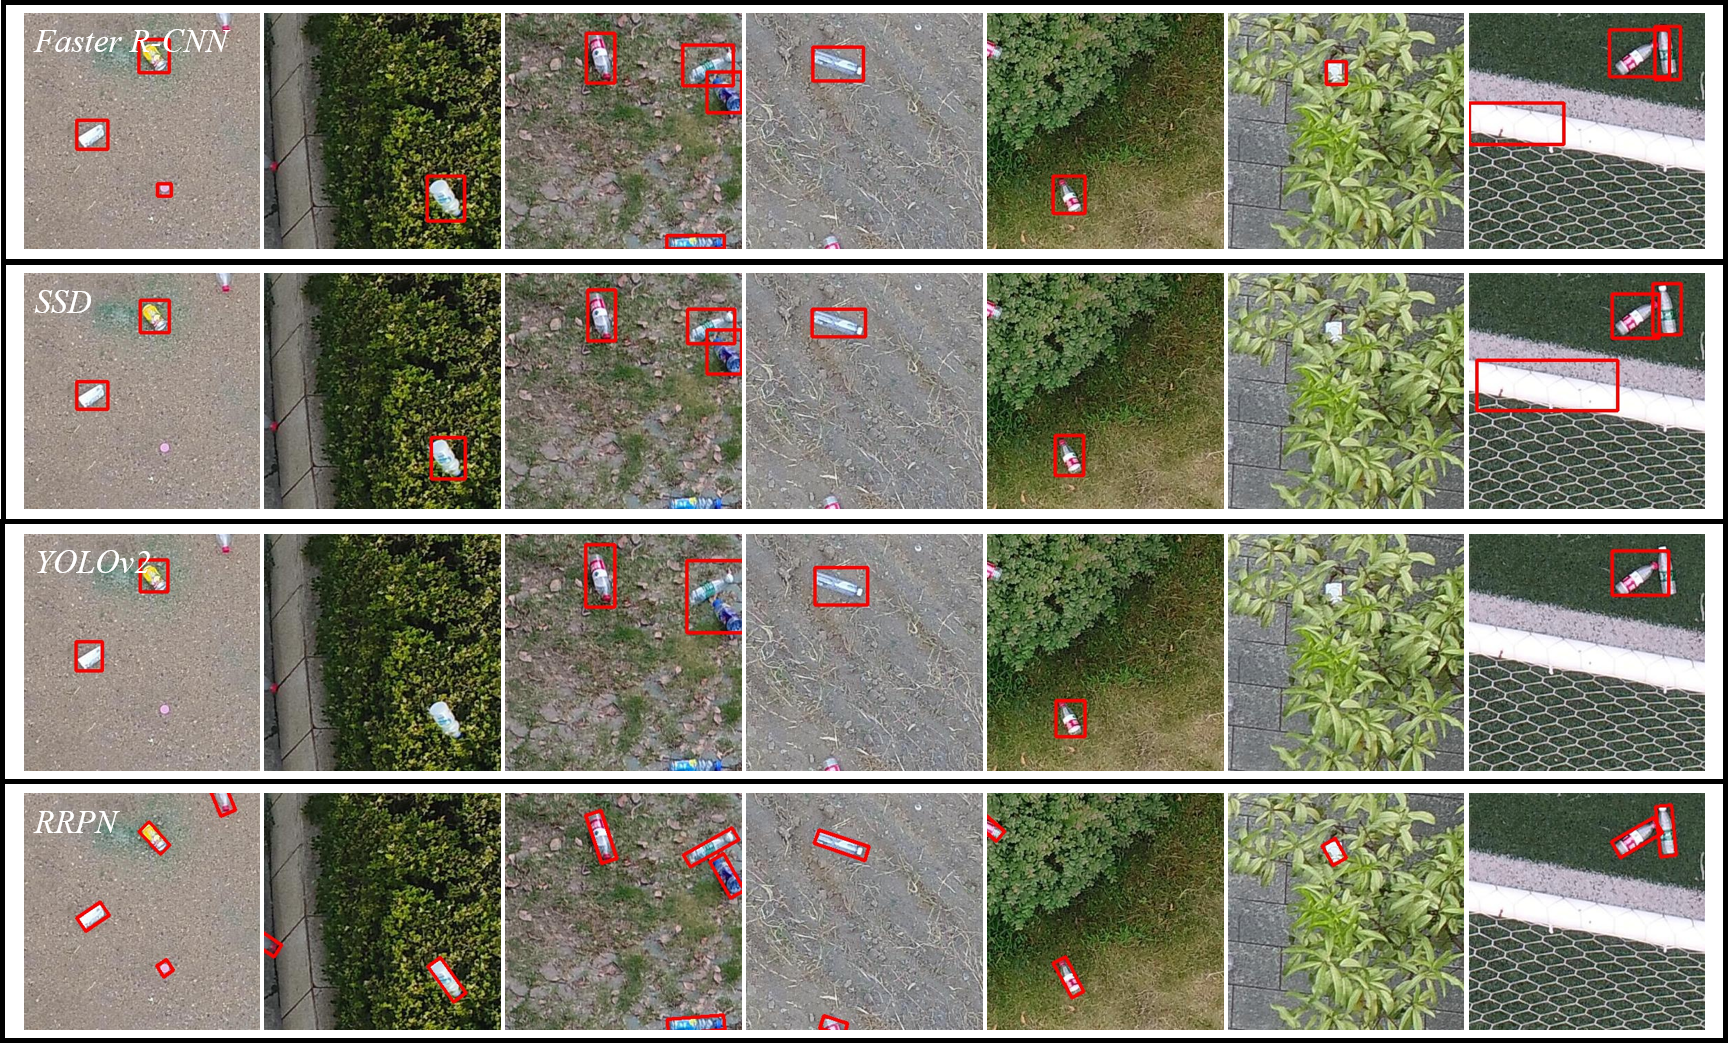
\includegraphics[width=\linewidth]{images/result.png}
	\caption{Visualization results of testing on UAV-BD using well-trained Faster R-CNN, SSD and RRPN. \textbf{Top} to \textbf{Bottom} respectively illustrate the results for Faster R-CNN, SSD, YOLOv2 and RRPN.}
	\label{fig:result}
\end{figure}


%\begin{figure}
%	\centering
%	\subfigure[angle distribution]
%	{
%		\label{angle}
%		\includegraphics[width=0.45\linewidth]{images/pr_bbox.pdf}
%	}
%	\subfigure[size distribution]
%	{
%		\label{size}
%		\includegraphics[width=0.45\linewidth]{images/pr_rbbox.pdf}
%	}
%	\caption{The precision-recall curve for bottle detection for Faster R-CNN, SSD and RRPN}
%	\label{fig:PR}
%\end{figure}


%\renewcommand{\algorithmicrequire}{\textbf{Input:}}
%\renewcommand{\algorithmicensure}{\textbf{Output:}}


%\begin{algorithm}
%	\caption{IoU computation}
%	\begin{algorithmic}[1]
%		\Require Rectangle $ R_1, R_2,\cdots,R_N $
%		\State IoU[1, $ N $][1, $ N $] $ \gets $ 0
%		\For {each pair of $ R_i, R_j(i<j) $} 
%		\State Point set $ PSet \gets \emptyset $
%		\State Add intersection points of $ R_i $ and $ R_j $ to $ PSet $
%		\State Add the vertices of $ R_i $ inside $ R_j $ into $ PSet $
%		\State $ \text{IoU}(i,j) \gets (\text{Area}(R_i) + \text{Area}(R_j) - I)/I $
%		\EndFor
%		\Ensure IoU
%	\end{algorithmic}
%\end{algorithm}

